\documentclass[reqno]{amsart} \usepackage{graphicx, amsmath, amssymb, amsfonts, amsthm, stmaryrd, amscd}
\usepackage[usenames, dvipsnames]{xcolor}
\usepackage{tikz}
% \usepackage{tikzcd}
% \usepackage{comment}

% \let\counterwithout\relax
% \let\counterwithin\relax
% \usepackage{chngcntr}

\usepackage{enumerate}
% \usepackage{enumitem}
% \usepackage{times}
\usepackage[normalem]{ulem}
% \usepackage{minted}
% \usepackage{xypic}
% \usepackage{color}


% \usepackage{silence}
% \WarningFilter{latex}{Label `tocindent-1' multiply defined}
% \WarningFilter{latex}{Label `tocindent0' multiply defined}
% \WarningFilter{latex}{Label `tocindent1' multiply defined}
% \WarningFilter{latex}{Label `tocindent2' multiply defined}
% \WarningFilter{latex}{Label `tocindent3' multiply defined}
\usepackage{hyperref}
% \usepackage{navigator}


% \usepackage{pdfsync}
\usepackage{xparse}


\usepackage[all]{xy}
\usepackage{enumerate}
\usetikzlibrary{matrix,arrows,decorations.pathmorphing}



\makeatletter
\newcommand*{\transpose}{%
  {\mathpalette\@transpose{}}%
}
\newcommand*{\@transpose}[2]{%
  % #1: math style
  % #2: unused
  \raisebox{\depth}{$\m@th#1\intercal$}%
}
\makeatother


\makeatletter
\newcommand*{\da@rightarrow}{\mathchar"0\hexnumber@\symAMSa 4B }
\newcommand*{\da@leftarrow}{\mathchar"0\hexnumber@\symAMSa 4C }
\newcommand*{\xdashrightarrow}[2][]{%
  \mathrel{%
    \mathpalette{\da@xarrow{#1}{#2}{}\da@rightarrow{\,}{}}{}%
  }%
}
\newcommand{\xdashleftarrow}[2][]{%
  \mathrel{%
    \mathpalette{\da@xarrow{#1}{#2}\da@leftarrow{}{}{\,}}{}%
  }%
}
\newcommand*{\da@xarrow}[7]{%
  % #1: below
  % #2: above
  % #3: arrow left
  % #4: arrow right
  % #5: space left 
  % #6: space right
  % #7: math style 
  \sbox0{$\ifx#7\scriptstyle\scriptscriptstyle\else\scriptstyle\fi#5#1#6\m@th$}%
  \sbox2{$\ifx#7\scriptstyle\scriptscriptstyle\else\scriptstyle\fi#5#2#6\m@th$}%
  \sbox4{$#7\dabar@\m@th$}%
  \dimen@=\wd0 %
  \ifdim\wd2 >\dimen@
    \dimen@=\wd2 %   
  \fi
  \count@=2 %
  \def\da@bars{\dabar@\dabar@}%
  \@whiledim\count@\wd4<\dimen@\do{%
    \advance\count@\@ne
    \expandafter\def\expandafter\da@bars\expandafter{%
      \da@bars
      \dabar@ 
    }%
  }%  
  \mathrel{#3}%
  \mathrel{%   
    \mathop{\da@bars}\limits
    \ifx\\#1\\%
    \else
      _{\copy0}%
    \fi
    \ifx\\#2\\%
    \else
      ^{\copy2}%
    \fi
  }%   
  \mathrel{#4}%
}
\makeatother
% \DeclareMathOperator{\rg}{rg}

\usepackage{mathtools}
\DeclarePairedDelimiter{\paren}{(}{)}
\DeclarePairedDelimiter{\abs}{\lvert}{\rvert}
\DeclarePairedDelimiter{\norm}{\lVert}{\rVert}
\DeclarePairedDelimiter{\innerproduct}{\langle}{\rangle}
\newcommand{\Of}[2]{{\operatorname{#1}} {\paren*{#2}}}
\newcommand{\of}[2]{{{{#1}} {\paren*{#2}}}}

\DeclareMathOperator{\Shim}{Shim}
\DeclareMathOperator{\sgn}{sgn}
\DeclareMathOperator{\fdeg}{fdeg}
\DeclareMathOperator{\SL}{SL}
\DeclareMathOperator{\slLie}{\mathfrak{s}\mathfrak{l}}
\DeclareMathOperator{\soLie}{\mathfrak{s}\mathfrak{o}}
\DeclareMathOperator{\spLie}{\mathfrak{s}\mathfrak{p}}
\DeclareMathOperator{\glLie}{\mathfrak{g}\mathfrak{l}}
\newcommand{\pn}[1]{{\color{ForestGreen} \sf PN: [#1]}}
\DeclareMathOperator{\Mp}{Mp}
\DeclareMathOperator{\Mat}{Mat}
\DeclareMathOperator{\GL}{GL}
\DeclareMathOperator{\Gr}{Gr}
\DeclareMathOperator{\GU}{GU}
\def\gl{\mathfrak{g}\mathfrak{l}}
\DeclareMathOperator{\odd}{odd}
\DeclareMathOperator{\even}{even}
\DeclareMathOperator{\GO}{GO}
\DeclareMathOperator{\good}{good}
\DeclareMathOperator{\bad}{bad}
\DeclareMathOperator{\PGO}{PGO}
\DeclareMathOperator{\htt}{ht}
\DeclareMathOperator{\height}{height}
\DeclareMathOperator{\Ass}{Ass}
\DeclareMathOperator{\coheight}{coheight}
\DeclareMathOperator{\GSO}{GSO}
\DeclareMathOperator{\SO}{SO}
\DeclareMathOperator{\so}{\mathfrak{s}\mathfrak{o}}
\DeclareMathOperator{\su}{\mathfrak{s}\mathfrak{u}}
\DeclareMathOperator{\ad}{ad}
% \DeclareMathOperator{\sc}{sc}
\DeclareMathOperator{\Ad}{Ad}
\DeclareMathOperator{\disc}{disc}
\DeclareMathOperator{\inv}{inv}
\DeclareMathOperator{\Pic}{Pic}
\DeclareMathOperator{\uc}{uc}
\DeclareMathOperator{\Cl}{Cl}
\DeclareMathOperator{\Clf}{Clf}
\DeclareMathOperator{\Hom}{Hom}
\DeclareMathOperator{\hol}{hol}
\DeclareMathOperator{\Heis}{Heis}
\DeclareMathOperator{\Haar}{Haar}
\DeclareMathOperator{\h}{h}
\def\sp{\mathfrak{s}\mathfrak{p}}
\DeclareMathOperator{\heis}{\mathfrak{h}\mathfrak{e}\mathfrak{i}\mathfrak{s}}
\DeclareMathOperator{\End}{End}
\DeclareMathOperator{\JL}{JL}
\DeclareMathOperator{\image}{image}
\DeclareMathOperator{\red}{red}
\def\div{\operatorname{div}}
\def\eps{\varepsilon}
\def\cHom{\mathcal{H}\operatorname{om}}
\DeclareMathOperator{\Ops}{Ops}
\DeclareMathOperator{\Symb}{Symb}
\def\boldGL{\mathbf{G}\mathbf{L}}
\def\boldSO{\mathbf{S}\mathbf{O}}
\def\boldU{\mathbf{U}}
\DeclareMathOperator{\hull}{hull}
\DeclareMathOperator{\LL}{LL}
\DeclareMathOperator{\PGL}{PGL}
\DeclareMathOperator{\class}{class}
\DeclareMathOperator{\lcm}{lcm}
\DeclareMathOperator{\spann}{span}
\DeclareMathOperator{\Exp}{Exp}
\DeclareMathOperator{\ext}{ext}
\DeclareMathOperator{\Ext}{Ext}
\DeclareMathOperator{\Tor}{Tor}
\DeclareMathOperator{\et}{et}
\DeclareMathOperator{\tor}{tor}
\DeclareMathOperator{\loc}{loc}
\DeclareMathOperator{\tors}{tors}
\DeclareMathOperator{\pf}{pf}
\DeclareMathOperator{\smooth}{smooth}
\DeclareMathOperator{\prin}{prin}
\DeclareMathOperator{\Kl}{Kl}
\newcommand{\kbar}{\mathchar'26\mkern-9mu k}
\DeclareMathOperator{\der}{der}
% \DeclareMathOperator{\abs}{abs}
\DeclareMathOperator{\Sub}{Sub}
\DeclareMathOperator{\Comp}{Comp}
\DeclareMathOperator{\Err}{Err}
\DeclareMathOperator{\dom}{dom}
\DeclareMathOperator{\radius}{radius}
\DeclareMathOperator{\Fitt}{Fitt}
\DeclareMathOperator{\Sel}{Sel}
\DeclareMathOperator{\rad}{rad}
\DeclareMathOperator{\id}{id}
\DeclareMathOperator{\Center}{Center}
\DeclareMathOperator{\Der}{Der}
\DeclareMathOperator{\U}{U}
% \DeclareMathOperator{\norm}{norm}
\DeclareMathOperator{\trace}{trace}
\DeclareMathOperator{\Equid}{Equid}
\DeclareMathOperator{\Feas}{Feas}
\DeclareMathOperator{\bulk}{bulk}
\DeclareMathOperator{\tail}{tail}
\DeclareMathOperator{\sys}{sys}
\DeclareMathOperator{\atan}{atan}
\DeclareMathOperator{\temp}{temp}
\DeclareMathOperator{\Asai}{Asai}
\DeclareMathOperator{\glob}{glob}
\DeclareMathOperator{\Kuz}{Kuz}
\DeclareMathOperator{\Irr}{Irr}
\newcommand{\rsL}{ \frac{ L^{(R)}(\Pi \times \Sigma, \std, \frac{1}{2})}{L^{(R)}(\Pi \times \Sigma, \Ad, 1)}  }
\DeclareMathOperator{\GSp}{GSp}
\DeclareMathOperator{\PGSp}{PGSp}
\DeclareMathOperator{\BC}{BC}
\DeclareMathOperator{\Ann}{Ann}
\DeclareMathOperator{\Gen}{Gen}
\DeclareMathOperator{\SU}{SU}
\DeclareMathOperator{\PGSU}{PGSU}
% \DeclareMathOperator{\gen}{gen}
\DeclareMathOperator{\PMp}{PMp}
\DeclareMathOperator{\PGMp}{PGMp}
\DeclareMathOperator{\PB}{PB}
\DeclareMathOperator{\ind}{ind}
\DeclareMathOperator{\Jac}{Jac}
\DeclareMathOperator{\jac}{jac}
\DeclareMathOperator{\im}{im}
\DeclareMathOperator{\Aut}{Aut}
\DeclareMathOperator{\Int}{Int}
\DeclareMathOperator{\PSL}{PSL}
\DeclareMathOperator{\co}{co}
\DeclareMathOperator{\irr}{irr}
\DeclareMathOperator{\prim}{prim}
\DeclareMathOperator{\bal}{bal}
\DeclareMathOperator{\baln}{bal}
\DeclareMathOperator{\dist}{dist}
\DeclareMathOperator{\RS}{RS}
\DeclareMathOperator{\Ram}{Ram}
\DeclareMathOperator{\Sob}{Sob}
\DeclareMathOperator{\Sol}{Sol}
\DeclareMathOperator{\soc}{soc}
\DeclareMathOperator{\nt}{nt}
\DeclareMathOperator{\mic}{mic}
\DeclareMathOperator{\Gal}{Gal}
\DeclareMathOperator{\st}{st}
\DeclareMathOperator{\std}{std}
\DeclareMathOperator{\diag}{diag}
\DeclareMathOperator{\Sym}{Sym}
\DeclareMathOperator{\gr}{gr}
\DeclareMathOperator{\aff}{aff}
\DeclareMathOperator{\Dil}{Dil}
\DeclareMathOperator{\Lie}{Lie}
\DeclareMathOperator{\Symp}{Symp}
\DeclareMathOperator{\Stab}{Stab}
\DeclareMathOperator{\St}{St}
\DeclareMathOperator{\stab}{stab}
\DeclareMathOperator{\codim}{codim}
\DeclareMathOperator{\linear}{linear}
\newcommand{\git}{/\!\!/}
\DeclareMathOperator{\geom}{geom}
\DeclareMathOperator{\spec}{spec}
\def\O{\operatorname{O}}
\DeclareMathOperator{\Au}{Aut}
\DeclareMathOperator{\Fix}{Fix}
\DeclareMathOperator{\Opp}{Op}
\DeclareMathOperator{\opp}{op}
\DeclareMathOperator{\Size}{Size}
\DeclareMathOperator{\Save}{Save}
% \DeclareMathOperator{\ker}{ker}
\DeclareMathOperator{\coker}{coker}
\DeclareMathOperator{\sym}{sym}
\DeclareMathOperator{\mean}{mean}
\DeclareMathOperator{\elliptic}{ell}
\DeclareMathOperator{\nilpotent}{nil}
\DeclareMathOperator{\hyperbolic}{hyp}
\DeclareMathOperator{\newvector}{new}
\DeclareMathOperator{\new}{new}
\DeclareMathOperator{\full}{full}
\newcommand{\qr}[2]{\left( \frac{#1}{#2} \right)}
\DeclareMathOperator{\unr}{u}
\DeclareMathOperator{\ram}{ram}
% \DeclareMathOperator{\len}{len}
\DeclareMathOperator{\fin}{fin}
\DeclareMathOperator{\cusp}{cusp}
\DeclareMathOperator{\curv}{curv}
\DeclareMathOperator{\rank}{rank}
\DeclareMathOperator{\rk}{rk}
\DeclareMathOperator{\pr}{pr}
\DeclareMathOperator{\Transform}{Transform}
\DeclareMathOperator{\mult}{mult}
\DeclareMathOperator{\Eis}{Eis}
\DeclareMathOperator{\reg}{reg}
\DeclareMathOperator{\sing}{sing}
\DeclareMathOperator{\alt}{alt}
\DeclareMathOperator{\irreg}{irreg}
\DeclareMathOperator{\sreg}{sreg}
\DeclareMathOperator{\Wd}{Wd}
\DeclareMathOperator{\Weil}{Weil}
\DeclareMathOperator{\Th}{Th}
\DeclareMathOperator{\Sp}{Sp}
\DeclareMathOperator{\Ind}{Ind}
\DeclareMathOperator{\Res}{Res}
\DeclareMathOperator{\ini}{in}
\DeclareMathOperator{\ord}{ord}
\DeclareMathOperator{\osc}{osc}
\DeclareMathOperator{\fluc}{fluc}
\DeclareMathOperator{\size}{size}
\DeclareMathOperator{\ann}{ann}
\DeclareMathOperator{\equ}{eq}
\DeclareMathOperator{\res}{res}
\DeclareMathOperator{\pt}{pt}
\DeclareMathOperator{\src}{source}
\DeclareMathOperator{\Zcl}{Zcl}
\DeclareMathOperator{\Func}{Func}
\DeclareMathOperator{\Map}{Map}
\DeclareMathOperator{\Frac}{Frac}
\DeclareMathOperator{\Frob}{Frob}
\DeclareMathOperator{\ev}{eval}
\DeclareMathOperator{\pv}{pv}
\DeclareMathOperator{\eval}{eval}
\DeclareMathOperator{\Spec}{Spec}
\DeclareMathOperator{\Speh}{Speh}
\DeclareMathOperator{\Spin}{Spin}
\DeclareMathOperator{\GSpin}{GSpin}
\DeclareMathOperator{\Specm}{Specm}
\DeclareMathOperator{\Sphere}{Sphere}
\DeclareMathOperator{\Sqq}{Sq}
\DeclareMathOperator{\Ball}{Ball}
\DeclareMathOperator\Cond{\operatorname{Cond}}
\DeclareMathOperator\proj{\operatorname{proj}}
\DeclareMathOperator\Swan{\operatorname{Swan}}
\DeclareMathOperator{\Proj}{Proj}
\DeclareMathOperator{\bPB}{{\mathbf P}{\mathbf B}}
\DeclareMathOperator{\Projm}{Projm}
\DeclareMathOperator{\Tr}{Tr}
\DeclareMathOperator{\Type}{Type}
\DeclareMathOperator{\Prop}{Prop}
\DeclareMathOperator{\vol}{vol}
\DeclareMathOperator{\covol}{covol}
\DeclareMathOperator{\Rep}{Rep}
\DeclareMathOperator{\Cent}{Cent}
\DeclareMathOperator{\val}{val}
\DeclareMathOperator{\area}{area}
\DeclareMathOperator{\nr}{nr}
\DeclareMathOperator{\CM}{CM}
\DeclareMathOperator{\CH}{CH}
\DeclareMathOperator{\tr}{tr}
\DeclareMathOperator{\characteristic}{char}
\DeclareMathOperator{\supp}{supp}


\theoremstyle{plain} \newtheorem{theorem} {Theorem} \newtheorem{conjecture} [theorem] {Conjecture} \newtheorem{corollary} [theorem] {Corollary} \newtheorem{proposition} [theorem] {Proposition} \newtheorem{fact} [theorem] {Fact}
\theoremstyle{definition} \newtheorem{definition} [theorem] {Definition} \newtheorem{hypothesis} [theorem] {Hypothesis} \newtheorem{assumptions} [theorem] {Assumptions}
\newtheorem{example} [theorem] {Example}
\newtheorem{assertion}[theorem] {Assertion}
\newtheorem{note}[theorem] {Note}
\newtheorem{conclusion}[theorem] {Conclusion}
\newtheorem{claim}            {Claim}
\newtheorem{homework} {Homework}
\newtheorem{exercise} {Exercise}  \newtheorem{question}[theorem] {Question}    \newtheorem{answer} {Answer}  \newtheorem{problem} {Problem}    \newtheorem{remark} [theorem] {Remark}
\newtheorem{notation} [theorem]           {Notation}
\newtheorem{terminology}[theorem]            {Terminology}
\newtheorem{convention}[theorem]            {Convention}
\newtheorem{motivation}[theorem]            {Motivation}


\newtheoremstyle{itplain} % name
{6pt}                    % Space above
{5pt\topsep}                    % Space below
{\itshape}                   % Body font
{}                           % Indent amount
{\itshape}                   % Theorem head font
{.}                          % Punctuation after theorem head
{5pt plus 1pt minus 1pt}                       % Space after theorem head
% {.5em}                       % Space after theorem head
{}  % Theorem head spec (can be left empty, meaning ‘normal’)

% \theoremstyle{mytheoremstyle}


\theoremstyle{itplain} %--default
% \theoremheaderfont{\itshape}
% \newtheorem{lemma}{Lemma}
\newtheorem{lemma}[theorem]{Lemma}
% \newtheorem{lemma}{Lemma}[subsubsection]

\newtheorem*{lemma*}{Lemma}
\newtheorem*{proposition*}{Proposition}
\newtheorem*{definition*}{Definition}
\newtheorem*{example*}{Example}

\newtheorem*{results*}{Results}
\newtheorem{results} [theorem] {Results}


\usepackage[displaymath,textmath,sections,graphics]{preview}
\PreviewEnvironment{align*}
\PreviewEnvironment{multline*}
\PreviewEnvironment{tabular}
\PreviewEnvironment{verbatim}
\PreviewEnvironment{lstlisting}
\PreviewEnvironment*{frame}
\PreviewEnvironment*{alert}
\PreviewEnvironment*{emph}
\PreviewEnvironment*{textbf}



\begin{document}

\title{Notes from 2024 Clay Research Conference}

\begin{abstract}
  Unedited notes from the talks of Ana Caraiani, Mark Andrea de Cataldo, Timothy Gowers, Rahul Pandharipande.  These notes are incomplete, have not been proofread, and should be considered only a crude approximation to what happened in the lectures, filtered through my own misunderstandings and distractions.  Any errors should be assumed to be due to the note-taker.
\end{abstract}

\maketitle

\tableofcontents

\part{Ana Caraiani (Imperial), \emph{The cohomology of Shimura varieties – a survey of recent developments}}

For this talk, we'll focus not on modularity, but instead on some really fascinating geometric objects that sometimes give you a concrete, explicit geometric realization of the Langlands correspondence, namely, Shimura varieties.  We'll thus talk about these fascinating objects and their many symmetries.  There's been much recent progress in the area.  Towards the end of the talk, we'll give some high level view on how some of the different talks at the workshop this week connect to each other.

To begin, we'll discuss Shimura varieties.

\section{Shimura varieties}

The global Langlands correspondence is supposed to match up different kinds of data showing up in different contexts.  On the harmonic analysis side, what you see are systems of eigenvalues that show up from the geometry or topology or analysis of certain highly symmetric spaces.  That's the perspective from which we'll approach Shimura varieties.  Later on, on the arithmetic side of the Langlands correspondence, we'll see the kind of data that comes from counting solutions to polynomial equations modulo primes.  But for now we'll focus on spaces with a lot of symmetry that know about a lot of interesting systems of eigenvalues.

These spaces will be attached to connected reductive groups $G$ over $\mathbb{Q}$ (e.g., $G = \GL_2$ or $\SL_2$).  We want to look at the so-called symmetric space $X$ for the real points of the group.  This is a real manifold endowed with a Riemannian metric.  We can just take $X = G(\mathbb{R}) / K_\infty^0 A_\infty^0$.  This definition makes sense over the reals, but we want something to reflect the structure that we started with over the rational numbers.  We get this by taking quotients.  The space $X$ has, by construction, a left action of $G(\mathbb{R})$.  If we had, for instance, started over $\mathbb{Z}$, then we could form the subgroup of integral points $\Gamma$ inside $G(\mathbb{R})$.  Shimura varieties are very roughly the locally symmetric spaces of the form $\Gamma \backslash X$ that arise in this way.  By taking $\Gamma$ sufficiently small (e.g., by imposing some congruences conditions), we can ensure that this quotient has the structure of a smooth real manifold.

This is just a first approximation -- Shimura varieties have additional structure.  One first piece of additional structure is what's called Hecke symmetry.  (This shows up even before you start talking about Shimura varieties.)  Take the finite adelic points $G(\mathbb{A}_f)$, given by the restricted product of the $G(\mathbb{Q}_p)$ for all primes $p$.  Arithmetic groups essentially arise by taking a small enough compact open subgroup $K \subset G(\mathbb{A}_f)$.  We then want to view our locally symmetric space not as a real quotient as above, but instead as a double quotient
\begin{equation*}
  X_K =
  G(\mathbb{Q}) \backslash  (X \times G(\mathbb{A}_f)) / K.
\end{equation*}
This is not so far apart from taking a disjoint union of real quotients as above.  More precisely, by strong approximation, we have
\begin{equation*}
  G(\mathbb{A}_f) = \sqcup_{
    \substack{
      i \in I  \\
      \text{finite set}      
    }
  }
  G(\mathbb{Q}) \gamma_i K,
\end{equation*}
and so
\begin{equation*}
  X_K = \sqcup_{i \in I} X / \Gamma_i , \qquad
  \Gamma_i = G(\mathbb{Q}) \cap \gamma_i K \gamma_i^{-1}.
\end{equation*}
This last construction of $X_K$ makes apparent the full force of symmetries available.  The right thing to do is to consider the inverse limit of these objects $X_K$ as $K$ gets smaller and smaller.  (It's sometimes useful to restrict to those $K$ that are unramified outside some finite set of primes.)  This inverse limit has a natural action of $G(\mathbb{A}_f)$.  Passing to cohomology, e.g.,
\begin{equation*}
  \varinjlim_{K} H^\ast(X_K, \mathbb{C}),
\end{equation*}
we retain an action of $G(\mathbb{A}_f)$.

We can remember the Hecke symmetry at finite level through the action of a Hecke algebra.  Namely, if you just want to look at some fixed finite level congruence subgroup $K$, then we can remember the symmetry coming from $G(\mathbb{A}_f)$ by considering the corresponding algebra of averaging operators $\mathbb{T}$, called the Hecke algebra.  We then obtain an action
\begin{equation*}
  \mathbb{T} \circlearrowright H^\ast(X_K, \mathbb{C}).
\end{equation*}

\section{Examples}

We'll now give one example and one non-example of Shimura varieties, followed by the general case.
\begin{enumerate}
\item\label{enumerate:cnpo4gcep4} $G = \GL_2$ over $\mathbb{Q}$.  The symmetric space is $X = \GL_2(\mathbb{R}) / \SO_2(\mathbb{R}) \mathbb{R}_{> 0}$, which we may identify with the disjoint union
  \begin{equation*}
    \mathbb{H}^{\pm} = \{ z \in \mathbb{C} : \Im(z) > 0 \text{ or } \Im(z) < 0\}
  \end{equation*}
  of upper and lower complex half-planes.  This identification comes from the action
  \begin{equation*}
    \gamma =
    \begin{pmatrix}
      a      & b \\
      c & d \\
    \end{pmatrix}
    \in \GL_2(\mathbb{R}).
  \end{equation*}
  That's the symmetric space; how about the locally symmetric space?  The $X_K$ are, by this approximation result, just disjoint unions of quotients $\Gamma \backslash \mathbb{H}$, where $\Gamma \subseteq \SL_2(\mathbb{Z})$ is a \emph{congruence subgroup}, namely, a finite-index subgroup cut out by congruence conditions.  There's a famous picture:
  \begin{figure}[h]
    \centering
    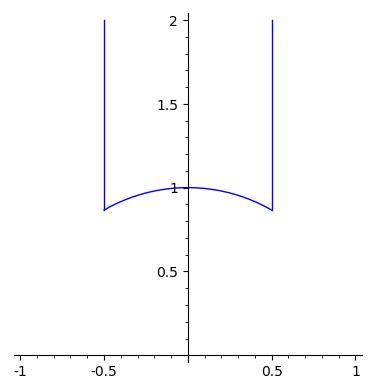
\includegraphics[width=0.5\textwidth]{fund-domain.png}
    \caption{Fundamental domain for $\SL_2(\mathbb{Z}) \backslash \mathbb{H}$}
    \label{fig:myimage}
  \end{figure}
  This looks like a punctured Riemann sphere, with a cusp at $\infty$ corresponding to the $y \rightarrow \infty$ limit and some orbifold-like points around the roots of unity $\rho = \exp(2 \pi i / 3)$ and $\rho^2$.

  So, this is a locally symmetric space, but in fact, even more happens in this example.  First of all, these are \emph{Riemann surfaces}, hence after compactifying at the cusps, they give rise to smooth projective curves over the complex numbers.  But what's even more special is that these curves can be defined by polynomial equations with \emph{rational} coefficients.

  Roughly speaking, Shimura varieties are locally symmetric spaces that admit an algebraic structure.

  A cohomology theory for algebraic varieties is the {\'e}tale cohomology, introduced by Grothendieck roughly 60 years ago.  This is supposed to behave kind of like the singular Betti  cohomology for topological spaces, but should compare while with de Rham cohomology.  We take our curve $S_K$ over the rational numbers and pass to its realization $S_K \times_{\mathbb{Q}} \bar{\mathbb{Q}}$ over the algebraic numbers, then take {\'e}tale cohomology with coefficients in $\mathbb{Q}_{\ell}$, and take the limit over $K$:
  \begin{equation*}
    H^\ast
    :=
    \varinjlim H^\ast_K
    :=
    \varinjlim_{K} H_{\acute{e}t}^\ast(S_K \times_{\mathbb{Q}} \bar{\mathbb{Q}}, \mathbb{Q}_{\ell}).
  \end{equation*}
  This retains the Hecke symmetry (an action of $\GL_2(\mathbb{A}_f)$) and a Galois symmetry (an action of $\Gal(\bar{\mathbb{Q}} / \mathbb{Q})$).

  Let's now get even more explicit.  Let $f$ be a cusp form of weight $2$.  It contributes to the cohomology $H^i$ in degree $i = 1$.  Writing $\mathfrak{m}_f$ for the Hecke ideal corresponding to the system of eigenvalues attached to $f$, we can identify $H^1_K[\mathfrak{m}_f]$ with the Galois representation attached to $f$, which we denote
  \begin{equation}\label{eq:cnpo4f57z3}
    \rho_{\mathfrak{m}, \ell} : G_{\mathbb{Q}} \rightarrow \GL_2(\bar{\mathbb{Q}}_{\ell}).
  \end{equation}
  We can also describe $H_K^0$.  If $\mathfrak{m} \subseteq \mathbb{T}$ occurs in it, then the corresponding Galois representation \eqref{eq:cnpo4f57z3} has the form $\chi(1 + \chi_{\mathrm{cycl}})$, where $\chi$ is a finite order character of $G_{\mathbb{Q}}$ and
  \begin{equation*}
    \chi_{\mathrm{cycl}} : G_{\mathbb{Q}} \rightarrow \Gal \left( \mathbb{Q}(\mu_{\ell^\infty}) / \mathbb{Q} \right) \cong \mathbb{Z}_{\ell}^\times
  \end{equation*}
  is the cyclotomic character.  Explicitly, if $p$ is a prime with $p \neq \ell$, then $\rho_{\mathfrak{m}, \ell}(\mathrm{Frob}_p)$ has eigenvalues $\{\alpha, \alpha p\}$.  This gives an example of the general phenomenon that cohomology away from the middle degree becomes degenerate.

\item\label{enumerate:cnpo4gb852} We now give a non-example.  Take an imaginary quadratic extension $F = \mathbb{Q}(\sqrt{- d})$, where $d > 0$ is square-free.  Take $G = \SL_2 / F$.  Let $X$ be a symmetric space for $G(\mathbb{R})$, which turns out to be identified with $\SL_2(\mathbb{C}) / \SU_2(\mathbb{R})$, which we may identify further with hyperbolic $3$-space $\mathbb{H}^3$.  This has odd real dimension, hence has no hope of having a complex structure.  Thus, here, $X_K$ are arithmetic hyperbolic $3$-manifolds, with no algebraic structure.  That's the general picture for locally symmetric spaces.
  
\item\label{enumerate:cnpo4ghhcx} What gave us an algebraic structure in example \eqref{enumerate:cnpo4gcep4} was that we started with a moduli space of elliptic curves with additional structure.  If we consider now $G := \GSp_{2 g}$ over $\mathbb{Q}$, then the corresponding Shimura varieties $S_K$ are moduli spaces of abelian varieties of dimension $g$, with principal polarizations and $K$-level structures.  There are other higher rank groups that give rise to Shimura groups, such as unitary groups, but they are special within the broader realm of reductive groups.  Anyway, the main point is that you have a Galois symmetry in addition to the Hecke symmetry.  These varieties are smooth and quasi-projective and defined over $\mathbb{Q}$ or some finite extension, and often, but not always, can be related to a moduli problem of abelian varieties with extra structure.  That's something that's very useful in their study -- the ones with this feature are often better understood than those without.  Because they have these additional symmetries, they are also good test objects for conjectures in arithmetic geometry.
\end{enumerate}

For the rest of the talk, we'll talk about the feature discussed above for $\GL_2$ where the most nondegenerate stuff occurs in middle degree, and away from that, one sees some degeneration.

\section{Intersection cohomology}

If you want a cohomology theory that is very well-behaved (e.g., satisfies Poincare duality) in the setting of varieties that are quasi-projective but not necessarily projective, then you can work with something called intersection cohomology.  Conjectures of Arthur and Kottwitz (from more than twenty years ago) predict what the intersection cohomology $\operatorname{IH}^\ast(S_K, \ast)$ of a Shimura variety should look like, over $\ast = \mathbb{C}$ or $\mathbb{Q}_{\ell}$.  There's a Lefschetz structure and a Hodge structure.  By looking at the interactions of these structures, one is led to the expectation that
\begin{equation*}
  \operatorname{IH}^{d - k}(S_K, \mathbb{Q}_{\ell}) \cong \operatorname{IH}^{d + k}(S_K, \mathbb{Q}_{\ell})
\end{equation*}
is more and more degenerate as $k$ grows.  Here $d = \dim S_K$.  In characteristic zero, one can approach these conjectures using known results toward functoriality.

In the rest of talk, we turn to the question: is there an analogue of Arthu's conjecture with torsion coefficients, e.g., for the intersection cohomology $\operatorname{IH}^\ast(S_K, \mathbb{F}_{\ell})$ with coefficients in a finite field?  Questions of this form have many applications, which will come up in the research workshop this week.  If you can put some nondegeneracy condition and know that cohomology will be concentrated in the middle degree, then this can be very useful for proving modularity theorems, the kinds of results useful for establishing the ``other direction'' of the Langlands correspondence.  This also plays a role in the prize-winning work of Newton--Thorne.  It also has applications to Euler systems, which are used to attack the BSD conjecture (Naomi Sweeting's talk yesterday at the workshop).  This kind of result has also played a key role in advances in understanding the Langlands correspondence in the Bianchi setting, such as in work of Caraiani--Newton.  It's also just interesting to see what the cohomology looks like in the torsion setting, to understand the analogues of conjectures originally formulated by Langlands.

To end, we'll describe a sample theorem in the compact case, and mention some work in progress specifically for intersection cohomology.  We give a sample result, informally stated.
\begin{theorem}[Sample theorem]
  Assume $S_K$ is compact.  Let $\mathfrak{m} \subseteq \mathbb{T}$ be a system of Hecke eigenvalues occurring in $H^\ast(S_K, \mathbb{F}_{\ell})$.  If $\mathfrak{m}$ is sufficiently generic (representation-theoretic condition at $p \neq \ell$, excluding cases like $\{\alpha, \alpha p\}$ discussed earlier), then
  \begin{equation*}
    H^\ast(S_K, \mathbb{F}_{\ell})_{\mathfrak{m}}
  \end{equation*}
  is concentrated in middle degree $d = \dim S_K$.
\end{theorem}
We didn't put attribution here, because it's a bit complicated.  The strategy for proving this is due to Caraiani--Scholze, then a better version was put forth by Koshikawa (a speaker on Monday), then an even stronger version put up last year by Hamann--Lee \cite{2023arXiv2309.08705}.  Results like this apply to most unitary Shimura varieties, and $\GSp_4$, but not quite in general, for various reasons.  The modern proof of the theorem uses the Igusa stack of M.\ Zhang, extended in work of Daniels--Kim--van Hoften--Zhang for more general Shimura varieties.  When you work over $p$-adic fields, namely, over $\mathbb{C}_p$, there is a Cartesian diagram
\begin{equation*}
  \begin{CD}         
    \mathcal{S}_{K^p}    @>>> \mathcal{H}_{G, \mu}\\
    @VVV  @VVV \\
    \mathrm{Igs} @>\bar{\pi}>> \mathrm{Bun}_G\\
  \end{CD}
\end{equation*}
due to work of various authors.  (Here $\mathrm{Igs}$ is the so-called Igusa stack.)  This gives a way to understand cohomology of Shimura varieties using ideas from the geometric Langlands program.  Namely, for well-behaved sheaves on $\mathrm{Bun}_G$, one has access to excursion operators, coming from Fargues--Scholze.  This leads to the most conceptual proof of the sample theorem.  The global input that you need is to know that the relative cohomology
\begin{equation*}
  R \bar{\pi}_\ast \mathbb{F}_{\ell}
\end{equation*}
is, in some sense, a perverse sheaf on $\mathrm{Bun}_G$.  One can recover
\begin{equation*}
  \varinjlim_{K_p} H^\ast(\mathrm{Sh}_{K^p K_p}, \mathbb{F}_{\ell})_{\mathfrak{m}}
\end{equation*}
by applying a Hecke symmetry $T_\mu$ to $(R \bar{\pi}_\ast \mathbb{F}_{\ell})_{\mathfrak{m}}$.  Then $T_\mu$ is perverse $t$-exact on a generic subcategory (coming from the work of Linus Hamann).  These themes will recur in the talks of Mingjia Zhang and Pol van Hoften.

We conclude by mentioning that in joint work, we are constructing an intersection complex on the Igusa stack that should recover the intersection cohomology of Shimura varieties, so you should have a theorem like the above (for middle degree) but instead for the intersection cohomology.  Depending upon the $t$-exactness properties of this Hecke operator on various subcategories, you could potentially realize the relative cohomology of the Igusa stack as a global incarnation of the generalized eigensheaves that showed up in Koshikawa's talk, and the analogue of Arthur's conjectures should be explained by $t$-exactness properties on smaller subcategories.

[applause]

\begin{remark}
  We understand what the points on $\mathrm{Bun}_G$ look like.  For instance, in $\GL_2$, the Igusa stack will reach two points, supersingular and ordinary, and the fibers will be more complicated objects called Igusa varieties.  The fibers of the map $\bar{\pi}$ are related to these.  What's really important about the Igusa stack is that it's kind of globalizing, giving a way to glue together these objects.  The moduli problem is abelian varieties but up to $p$-power isogeny.
\end{remark}


\part{Mark Andrea de Cataldo (Stony Brook), \emph{The $P=W$ Conjecture in Non Abelian Hodge Theory}}


The topic of the workshop is the $P = W$ conjecture in non-abelian Hodge theory.  The purpose of this hour is to introduce that conjecture.
\begin{itemize}
\item First, we'll say what non-abelian Hodge theory is.  
\item The $P = W$ conjecture then has two parts: $P$ and $W$.
\item We'll then state the conjecture, report on the status of the conjecture, and give some concluding remarks.
\end{itemize}

Before non-abelian Hodge theory, there is of course abelian Hodge theory.  Today ``abelian'' refers to $\GL_1 = \mathbb{C}^\times$, while ``non-abelian'' refers to $\GL_r$ with $r > 1$.

Let $X$ be a curve, with genus $g \geq 2$.  The main object today will be an $H^1$.  In the abelian case, we'll get a Lie group, but in the non-abelian case, we won't get a Lie group, but we'll instead get a complex algebraic variety that we'll study on its own terms.  The $H^1$ of interest will be
\begin{equation*}
  H^1(X, \mathbb{C}^\times) =
  \frac{H^1(X, \mathbb{C})}{H^1(X, \mathbb{Z})}.
\end{equation*}
We can think of this as $\Hom(\pi_1(X), \mathbb{C}^\times)$ (later, we'll need to work with an equivalence relation, but that relation is trivial here because the group $\GL_1$ is abelian).  It is isomorphic to $(\mathbb{C}^\times)^{2 g}$.  It is a complex algebraic variety, and is affine -- it can be embedded as a closed subvariety of some finite-dimensional affine space.  We can think of this further as the character variety $M_B(X, \GL _1)$ (here $B$ stands for ``Betti'').

There are ways to describe cohomology, and we have the de Rham theorem.  We can view the above quotient as
\begin{equation*}
  \frac{H^1_{d R}(X, \mathbb{C})}{H^1(X, \mathbb{Z})},
\end{equation*}
but we can then put connections on $X \times \mathbb{C}$, and the above quotient then identifies with
\begin{equation*}
  \frac{  \left( \frac{\text{closed forms}}{\text{exact forms}} \right)}{
    H^1(X, \mathbb{Z})
  }
  =
  \frac{\text{flat connections on $X \times \mathbb{C}$}}{\text{gauge}}.
\end{equation*}
We can also define $M_{d R}(X, \GL_1)$.  It is also a complex Lie group, but we want to emphasize that the relation between these two is not always so simple.  There is a biholomorphism
\begin{equation*}
  M_{d R}(X, \GL_1) \cong M_B(X, \GL_1).
\end{equation*}
That is to say, as complex analytic spaces, these are the same.  But if defined correctly, the left hand side is not affine, while the right hand side is affine.  (There are no polynomial functions on the left, but there are on the right.)

There's something you can do when you have a connection $D$: you can write it as a closed connection $D_0$ plus a form $\eta$, thus $D = D_0 + \eta$.  There is a canonical metric associated to a flat connection.  From this, we get an essentially canonical harmonic metric $H$.  You can take the
\begin{itemize}
\item the real part $\Re(\eta)$ and its $(1,0)$ part, and
\item the imaginary part $\Im(\eta)$ and its $(0,1)$ part.
\end{itemize}
From $\eta$ and $H$ we extract holomorphic connections
\begin{equation*}
  L_{\mathrm{dR}, \nabla^{\mathrm{hol}}}, \quad
  L_{\mathrm{Dol}, a},
\end{equation*}
where $a$ is a holomorphic $1$-form.  We obtain $M_{d R} \rightarrow \Jac(X)$, whose fibers are holomorphic $1$-forms $\Omega$.

We get a vector bundle $\Omega$ given by
\begin{equation*}
  \begin{CD}
    M_{\mathrm{Dol}}(X, \GL_1)    @>>>\Jac(X)\\
    @|  @. \\
    T^\ast \Jac(X) @>>> \Jac \Omega\\
  \end{CD}
\end{equation*}
\begin{equation*}
  H^1_{\mathrm{d R}} = \bar{\Omega} \oplus \Omega = \Jac(X) \times \Omega.
\end{equation*}
and $M_{\mathrm{Dol}} \cong M_{\mathrm{d R}}$ in the smooth category, but not biholomorphically.

We turn now to $\GL_r$.  We again have an affine algebraic variety
\begin{equation*}
  M_B(X, \GL_r) = \Hom(\pi_1, \GL_r) / \operatorname{conj} \GL_r.
\end{equation*}
There's also the de Rham side
\begin{equation*}
  M_{\mathrm{d R}}(X, \GL_r) =
  \frac{\text{rank $r$ hol.\ v.\ bundles on $X$}, \nabla : E \rightarrow E \otimes T_X^\ast}{\text{isom}}.
\end{equation*}
The third object is the Dolbeaut moduli space
\begin{equation*}
  M_{\mathrm{Dol}}(X, \GL_r) =
  \frac{\text{rank $r$ hol.\ v.\ bundles on } X, E : \xrightarrow{a} E \otimes T_X^\ast}{
    \text{isom}
  },
\end{equation*}
where now $a$ is merely a linear map rather than a connection.

These are three \emph{a priori} different algebraic varieties (and indeed, different already in rank one), but bearing the same relations as in the abelian case.  These are singular now, whereas before they were complex Lie groups.  What happens here is that $M_{\mathrm{d R}}$ and $M_{\mathrm{Dol}}$ are canonically homeomorphic (using that $H$ is harmonic, due to Carlette), while $M_B$ and $M_{\mathrm{d R}}$ are biholomorphic, via holonomy.  This is the content of the non-abelian Hodge theorem, due to Hitchin for $\SL_2$, contribution concerning $H$ due to Carlette, putting it together by Carlos Simpson; established in the late 80's, early 90's (and established thus far under some non-singularity assumptions: $d = c_1 E$, $(r, d) = 1$).

We saw earlier that you can take a Riemann surface $X$ and study its cohomology group $H^1(X, \mathbb{C})$ and its various moduli space $M$, which today we study from the point of view of singular cohomology $H^\ast(M)$.  The $P = W$ conjecture is about studying the singular cohomologies of these spaces when we look at them through the optics of their different structures.

$W$ stands for ``weight'', coming from the mixed Hodge theory due to Deligne.  We consider a smooth projective manifold $Y$, and work with $\mathbb{C}$ coefficients.  Then
\begin{equation*}
  H^k(Y, \mathbb{C}) = \oplus_{p + q = k}
  H^{p, q}(Y),
\end{equation*}
which we call a \emph{pure weight} $k$ \emph{Hodge structure}.  Now Deligne discovered that if we drop ``smooth'' and ``projective'' and instead consider merely quasi-projective $Y$, then the cohomology $H^k(Y, \mathbb{C})$ does not admit such a decomposition, but admits a weight filtration
\begin{equation*}
  W_0 \subset W_1 \subset \dotsb \subset W_{2 k} = H^k.
\end{equation*}
This is functorial with respect to $Y \rightarrow Y'$.  We get graded quotients
\begin{equation*}
  \operatorname{Gr}_w^W H^k
  =
  W_w / W_{w - 1}
  = \oplus_{p + q = w} H^{p, q}.
\end{equation*}

For example, consider the variety $\mathbb{C}^\times$.  We can then consider the space $H^1(\mathbb{C}^\times, \mathbb{C})$ or $H^1(\mathbb{C}^\times, \mathbb{Q})$.  In either case, the space is generated by $d z / z$, and coincides with $H^{1, 1}$ when $w = 2$.  We can realize the space as the kernel of
\begin{equation*}
  H^2(\mathbb{P}^1)^{\oplus 2} \rightarrow H^2 \mathbb{P}^1.
\end{equation*}
Comparing weights suggests why we call this ``mixed''.

To study $(\mathbb{C}^\times )^{2 g}$, we can use Kunneth.

We spent a lot of time with the three moduli spaces, but the $P = W$ conjecture is really about Betti and Dolbeault, so we now abandon the space $M_{d R}$.

Now, the cohomology of $M_{B}(X, \GL_r)$ is known to have a relatively simple structure:
\begin{equation*}
  H^k(M_B(X, \GL_r))
  = \oplus_{
    \substack{
      0 \leq w \leq 2 k  \\
      \text{$w$: even}      
    }
  }
  H^{w, w}(M_B).
\end{equation*}
\begin{itemize}
\item $\GL_2$: Hausel--R-Villegas
\item $\GL_r$: Shendl
\end{itemize}
Here $W = W_B$ on $H(M_B(X, \GL_r))$.

We now consider $P$ perverse.  The easier way to enter is via $D$-modules via the Riemann--Hilbert correspondence.  We can then understand the topology, through the work of Goresky--Macpherson and BBDG.  If you have a morphism of varieties $h : M \rightarrow A$, then we get a Leray filtration of spectral sequences on the singular cohomology $H(M)$ of the domain.  Now let's pretend that $h$ is a fiber bundle, just to give a face to this filtration.  Turn $A$ into a cell complex, so that the fiber bundle is trivial on the cell.  Take $A_K$, form its preimage $h^{-1}(A_K)$, its cohomology, the restriction map, and its kernel:
\begin{equation*}
  L = \ker \left( H^d(M) \rightarrow H^d(h^{-1}(A_K)) \right).
\end{equation*}
This is the standard 1950's way to look at the Leray spectral sequence.  Now, one reason why we wrote the paper like this is because we are going to consider a ``Hitchin map'' from the Dolbeaut moduli space
\begin{equation*}
  M_{\mathrm{Dol}} \xrightarrow{h} \mathbb{C}^{\frac{\dim M}{2}}(E, a),
\end{equation*}
where
\begin{equation*}
  E \xrightarrow{a} E,
\end{equation*}
what's called the spectral cover associated with $(E, a)$.  The map $h$ is proper, and is equivariant with respect to a certain $\mathbb{C}^\times$ action.  Everything retracts to zero in such a way that the Leray filtration $L_h$ is zero.  It's simple to deduce that the weight filtration on $W_{\mathrm{Dol}}$ is also trivial.

Now let's look at the cohomology on the Betti moduli space and the Dolbeault moduli spaces.  The isomorphisms between these spaces, given by the non-abelian Hodge theorem, give isomorphisms between their cohomology.  The $P = W$ conjecture asks, what corresponds on the Dolbeault side to the filtration $M_B$ on the Betti side?  It can't be either $W_{\mathrm{Dol}}$, or the Leray filtration $L_h$.

Let $P$ on $H^{\cdot}(M, \mathbb{Q})$ be formal.  There is a geometric description via the Lefschetz hyperplaen theorem.  We can take the Dolbeaut moduli space and the Hitchin map $h : M_{\mathrm{Dol}} \rightarrow \mathbb{C}^N$.  We can restrict this to the preimage $h^{-1}(\mathbb{C}^k)$ of $\mathbb{C}^k \subseteq \mathbb{C}^N$.  This induces a map in cohomology, whose kernel describes $P$:
\begin{equation*}
  P_p H^d(M_{\mathrm{Dol}}) = \ker ( H^d(M_{\mathrm{Dol}}) \rightarrow H^d (h^{-1}(\mathbb{C}^{d-p-1}))).
\end{equation*}

\begin{conjecture}[$P = W$, de Cataldo--Hausel--Migliorini, 2008]
  Under the isomorphism in cohomology coming from the non-abelian Hodge theorem, we have
  \begin{equation*}
    H^\ast M_{\mathrm{Dol}} \leftrightarrow H^\ast M_B,
  \end{equation*}
  \begin{equation*}
    P_p \leftrightarrow W_{2 p}.
  \end{equation*}
\end{conjecture}
\begin{theorem}[$P=W$ for Riemann surfaces $X$, $\GL_r$, coprime case; 2022: Maulik--Shen, Hausel--Mellit--Minets--Schiffmann; 2023: Maulik--Shen--Yin]
  .
\end{theorem}

It seems that this $P = W$ phenomenon is not just restricted to the contents of the non-abelian Hodge theorem, but occurs, but work of many people, in different setups, such as in mirror symmetry, cluster varieties, geometric depth and combinatorics, and the study of complex hyper K\"{a}hler varieties.  Somehow $P = W$ seems to be true in many cases.

Having stated the conjecture, let's make some concluding remarks.  We take $\dim X \geq 1$, and $G$ a reductive group.  In this case, the varieties are always singular, so the cohomology we'll work with is always the intersection cohomology $\mathrm{IH}^\ast$.  Two theorems are relevant.

\begin{itemize}
\item One is relative hard Lefschetz.  Hard Lefschetz says that for a smooth projective variety $Y$ and $\eta = c_1(A)$ on $X$, with $A$ ample, we have
  \begin{equation*}
    H^{n - k} \xrightarrow[\cong]{\eta^k} H^{n + k}.
  \end{equation*}
  Relative Hard Lefschetz (BBDG, Saito) says that
  \begin{equation*}
    \operatorname{Gr}^p_{\dim M - k} H^d M_{\mathrm{Dol}} \xrightarrow{\eta^k}
    \operatorname{Gr}^p_{\dim M + k} H^{d + 2 k} M_{\mathrm{Dol}},
  \end{equation*}
  with $\eta \in H^2 M_{\mathrm{Dol}}$ corresponding to $\eta \in H^2 M_B$ ($H^{1, 1}$ vs.\ $H^{2, 2}$).
\item The other is the curious hard Lefschetz, which says
  \begin{equation*}
    \Gr^W_{2 \dim M - 2 k} H^d M_{B} \xrightarrow[\cong]{\eta^k}
    \operatorname{Gr}^W_{2 \dim M + 2 k} H^{d + 2 k} M_B .
  \end{equation*}
  For $\GL_2$, this is Hausel--R-Villegas.  For $\GL_r$, Mellit.  The proofs don't give a fundamental reason why this should be true, and it would be interesting to obtain such a reason.
\end{itemize}

\part{Timothy Gowers (Cambridge), \emph{Some recent developments in combinatorics}}

Lots of recent progress that we highlight here.

Criteria for inclusion:
\begin{itemize}
\item Proved in the last five years.
\item ``Notable'' (e.g., reported in Quanta)
\item Solved a problem that people didn't expect to be solved any time soon.
\item (Proved by ``new entrants''.)
\end{itemize}

\section{Ramsey's theorem}

\begin{theorem}[Ramsey's theorem]
  For every $k$ and $l$, there exists $n$ such that every graph with $n$ vertices contains a clique of size $k$ or an independent set of size $l$.
\end{theorem}

The smallest such $n$ is the Ramsey number $R(k, l)$.


\begin{theorem}[Ramsey's theorem, equivalent formulation]
  For every $k$ and $l$, there exists $n$ such that if the edges of the complete graph with $n$ vertices are colored red or blue, then there is a clique of size $k$ with all its edges red or all its edges blue.
\end{theorem}
\begin{proof}[Proof sketch]
  Let the vertices be $v_1, \dotsc, v_N$ with $n = 2^{2 k}$.

  Find $i_1 < \dotsb < i_{2 k}$ such that if $r < s$, then the color of the edge $v_{i_r} v_{i_s}$ depends only on $i_r$.

  Do this inductively, choosing $v_{i_1}, \dotsc, v_{i_{2 k}}$ and $V_{i_1} \supset \dotsb \supset V_{i_{2 k}}$ such that for each $t$, we have that $v_{i_t}$ is the minimal element of $V_{i_{t - 1}}$, all edges from $v_{i_t}$ to $V_{i_t}$ have the same color, and $\lvert V_{i t} \rvert \geq 2^{2 k - t}$.

  Now from the vertices $v_{i_1}, \dotsc, v_{i_{2 k}}$, choose $k$ of them such that the color in question is the same for each one.
\end{proof}

The argument shows that $R(k, k) \leq 4^k$.  A tighter version due to Erdos and Szekeres gives an upper bound of
\begin{equation*}
  \binom{2(k - 1)}{ k - 1} = \O(4^k / \sqrt{k}).
\end{equation*}
Lower bound: $R(k, k) \geq 2^{k /2}$.  (In fact, one can do slightly better than this.)

\begin{proof}[Sketch of proof]
  Pick a red/blue coloring of the edges of $K_n$ at random.  Calculate that if $n \leq 2^{k/2}$, then the expected number of monochromatic cliques of size $k$ is strictly less than $1$.
\end{proof}

There's an exponential size gap between this $4^k / \sqrt{k}$ and $2^{k /2}$, each given by rather straightforward arguments, so it became very tempting to try to close that gap.
\begin{itemize}
\item What is $\lim_{k \rightarrow \infty} R(k, k)^{1/k}$?
\item Does it even exist?
\item Previous progress of R{\"o}dl, Thomason, Conlon, Sah -- quasirandomness.
\item Is $\limsup_{k \rightarrow \infty} R(k, k)^{1/k} < 4$?
\item Is $\liminf_{k \rightarrow \infty} R(k, k)^{1/k} > \sqrt{2}$?
\end{itemize}
These last questions were open until 16th March 2023, when Campos, Griffiths, Morris and Sahasrabudhe proved
\begin{equation*}
  R(k, k) \leq 4^k e^{- k / 80 + o(k)}.
\end{equation*}
Here we note that $4 \exp(-1/80) = 3.9503112 \dotsc$

Rather than quasirandomness, they used a delicate elementary approach via finding monochromatic ``books''.  (A \emph{book} is a graph with vertex set $R \cup S$ that contains all edges with at least one vertex in $S$.)

Let's quickly look at $R(k, l)$, where $k$ is \emph{fixed}.  Essentially the same arguments as above give
\begin{equation*}
  R(3, k) = k^2 \text{ up to log factors},
\end{equation*}
\begin{equation*}
  k^{5/2} \leq R(4, k) \leq k^3 \text{ up to log factors.}
\end{equation*}
The log factors for $R(3, k)$ have now been removed and we know that $R(3, k) = k^2 / \log k$ up to a constant.  (Upper bound by Ajtai, Komlos and Szemeredi in 1980, lower bound by Kim in 1995.)  But the $R(4, k)$ gap is bigger, and was very stubborn.

6th June 2023, Mattheus and Verstraete:
\begin{equation*}
  R(4, k) = \Omega(k^3 / \log^4 t).
\end{equation*}
Compares with the AKS upper bound of $\O(k^3 / \log^2 t)$.  They randomly sample from algebraically constructed structures with special properties.

\section{Arithmetic progressions of length $3$}

\begin{theorem}[Szemeredi, 1975]
  For every $\delta > 0$ and $k \in \mathbb{N}$, there exists $n \in \mathbb{N}$ such that every subset $A$ of $\{1, \dotsc, n\}$ of size at least $\delta n$ contains an arithmetic progression of length $k$.  
\end{theorem}

The case $k = 3$ was proved by Roth in 1953, who showed that $A$ contains a 3AP if $\delta \geq C / \log \log n$.  A lot of subsequent work was devoted to improving this bound (Szemeredi, Heath--Brown, Bourgain, Sanders, Bloom, Schoen), getting to $(\log \log n)^{3 + o(1)} / \log n$.

A lower bound of $\exp(- c \sqrt{\log n})$ proved by Behrend in 1946.  Small refinement due to Elkin, given a simpler proof by Green and Wolf.  Recently the constant $c$ improved by Elsholtz, Hunter, Proske and Sauermann.  Still leaves a big gap.

7th July 2020: Bloom and Sisask obtained a bound of $1 /(\log n)^{1 + c}$ for some positive $c$.

10th February 2023: Kelley and Meka improved this to a Behrend-style bound of $\exp(- c(\log n)^\beta)$.  We now know that $\beta$ can be taken to be $1/11$.  The proof was surprising not that bad.

\section{The inverse theorem for the uniformity norms}

One way to prove Szemeredi's theorem is as follows.  Given a subset $A \subset \{1, \dotsc, n\}$ of density $\delta$, identify $\{1, \dotsc, n\}$ with $\mathbb{Z} / n  \mathbb{Z}$ and define $f : \mathbb{Z} / n \mathbb{Z} \rightarrow \mathbb{R}$ by
\begin{equation*}
  f(x) =
  \begin{cases}
    1 - \delta &  x \in A \\
    - \delta               & \text{ otherwise}.
  \end{cases}
\end{equation*}
Then $A$ contains roughly the same number of $k$APs as a random set (i.e., around $\delta^k n^2$) if $f$ is small in a certain norm, called the $U^{k - 1}$-norm.

What does the $U^k$ norm look like when $k = 3$?
\begin{align*}
  &\lVert f \rVert_{U^3}^8 \\
  &= \mathbb{E}_{x, a,b,c}
    f(x) \overline{f(x - a) f(x - b) f(x - c)}
    f(x - a - b)
    f(x - b - c)
    f(x - a - c)
    \overline{f(x - a - b - c)}.
\end{align*}

We then need to understand what $f$ (and hence $A$) is like if $\lVert f \rVert_{U^k}$ is large.  For that, we need \emph{inverse theorems} for the $U^k$ norm.

\begin{theorem}[Weak inverse theorem]
  If $\lVert f \rVert_\infty \leq 1$ and $\lVert f \rVert_{U^k} \geq c$, then there is a polynomial $\phi$ of degree $k - 1$ and an arithmetic progression $P$ of length tending to infinity with $n$ such that
  \begin{equation*}
    \left| \mathbb{E}_{x \in P} f(x) \exp(- 2 \pi i \phi(x) / n) \right| \geq \alpha(c).
  \end{equation*}
\end{theorem}
Passing to a subprogression was necessary because of ``generalized polynomials''.  (Example: given $x$ we write it as $a + b m$ where $m \approx \sqrt{n}$ and $a, b \leq m$, and then let $\phi(x) = r a^2 + s a b + t b^2$.)

Green and Tao gave a precise formulation of ``generalized polynomial'' in terms of nilmanifolds in 2006, motivated by the wish to generalize and strengthen the Green--Tao theorem

\begin{conjecture}[loosely stated]
  If $\lVert f \rVert_{U^k}$ is not small, then $f$ correlates with a generalized polynomial phase function.
\end{conjecture}

Green, Tao and Ziegler proved this conjecture in 2010, but their proof did not give bounds (though in principle, with a lot of work, one could extract a very weak bound).

In 2018, Manners gave a new proof of the theorem, obtaining a doubly exponential dependence (of the correlation with the generalized polynomial phase function on $k$ and the size of the $U^k$ norm).  Already very notable as the proof introduced many interesting ideas and gave the first reasonable bound.

28th February 2024: James Leng, Ashwin Sah and Mehtaab Sawhney proved a \emph{quasipolynomial} dependence.  Oversimplifying slightly, this gives a dependence of the form $\alpha(c) = \exp(- \log(1/c)^{\O(1)})$.  This has several applications, including significantly improved bounds for Szemeredi's theorem, and simpler proofs of several other known theorems.

\section{The expectation threshold conjecture}

Let $G$ be a graph with $n$ vertices.  A \emph{Hamilton cycle} is an ordering $v_1, \dotsc, v_n$ of the vertices such that $v_1 v_2, v_2 v_3, \dotsc, v_{n - 1} v_n, v_n v_1$ are all edges.

If $G$ is a random graph where each edge is chosen independently with probability $p =p(n)$, then how large does $p$ have to be before
\begin{equation*}
  \mathbb{P}[\text{$G$ contains a Hamilton cycle}] \geq 1/2?
\end{equation*}
KS (Komlos and Szemeredi) showed it's about $(\log n + \log \log n) / n$, and a corresponding ``hitting time'' result.  We call this the \emph{threshold probability} for the problem.

Alternatively, what is the expected number of Hamilton cycles if each edge is chosen with probability $p$?  The number of cyclic orderings of the vertices is $(n - 1)!$.  Each one has a probability $p^n$ of giving rise to a Hamilton cycle.  So it is $p^n(n - 1)!$.

If the probability of having a Hamilton cycle is at least $1/2$, then the expected number of Hamilton cycles is at least $1/2$.  Is there anything resembling a converse to this implication?  No obvious reason, but by staring at examples, one sees that they do seem to be the same up to logarithmic factors.

A simple back-of-envelope calculation shows that in order for $p^n(n - 1)!$ to be at least $1/2$, we need $p$ to be around $e /n$.  This is (lying a little) the \emph{expectation threshold} for the problem.  Since the actual threshold was about $\log n / n$, the expectation threshold is off by a factor $\log n$.

\begin{conjecture}[Kahn, Kalai, 2006]
  For all monotone graph properties, the threshold is at most $\log n$ times the expectation threshold.
\end{conjecture}

Here's a quick indication of how to generalize it.  Take an increasing family $\mathcal{F}$ of subsets of $\{1, \dotsc, n\}$.  Choose a random subset $A$ of $\{1, \dotsc, n\}$ by picking each element independently with probability $p$.

The \emph{threshold} for $\mathcal{F}$ is the $p$ at which $\mathbb{P}[A \in \mathcal{F}]$ passes $1/2$.

We say that $\mathcal{F}$ is $p$\emph{-small} if there is a family $\mathcal{G}$ with the following two properties.
\begin{enumerate}
\item For each $F \in \mathcal{F}$, there exists $G \in \mathcal{G}$ such that $G \subset F$.
\item We have $\sum_{G \in \mathcal{G}} p^{\lvert G \rvert} \leq 1/2$.
\end{enumerate}
If $A$ is chosen randomly as above, then
\begin{equation*}
  \mathbb{P}[G \subset A] = p^{\lvert G \rvert},
\end{equation*}
so
\begin{equation*}
  \mathbb{P}[A \in \mathcal{F}]
  \leq \mathbb{P}[G \in \mathcal{G}, \,G \subset A]
  \leq \sum_{G \in \mathcal{G}} p^{\lvert G \rvert} \leq 1/2.
\end{equation*}

The expectation threshold cojecture is that the resulting thresholds coincide up to mild factors.

22nd August 2019: Alweiss, Lovett, Wu, Zhang: huge improvement to the bounds for the Erdos--Rado sunflower lemma, introducing the important new notion of a $q$-spread probability measure.

29th October 2019: Frankston, Kahan, Narayanan, Park

31 March 2022: Park, Pham, beautiful $4$-page proof.

Still open: do the expectation threshold and fractional expectation threshold agree up to a constant factor?


\section{The Erdos--Hajnal conjecture}
Let $H$ be a fixed graph.  If we add the hypothesis that a graph $G$ does not contain an induced copy of $H$, then by how much can we improve the bound in Ramsey's theorem?

\begin{conjecture}[Erdos and Hajnal, 1977]  For every $H$, there exists $\delta > 0$ such that if $G$ has $n$ vertices and does not contain an induced copy of $H$, then $G$ has a clique or independent set of size at least $n^\delta$.
\end{conjecture}
Known for some simple families of graphs and one or two small graphs.  The following special case was the simplest that was open:
\begin{question}
  Is the new Erdos--Hajnal conjecture true when $H$ is a pentagon?
\end{question}

9th February 2021: Chudnovsky, Scott, Seymour and Spirkl proved several new cases of the conjecture, including that of the pentagon.  Ties in with a major and very active theme of model theory.

\section{The union-closed conjecture}

\begin{conjecture}[Frankl, 1979] Let $\mathcal{A}$ be a finite family of sets that is closed under taking unions.  Then (except in the trivial case $A = \{\emptyset\}$), there is an element $x$ that belongs to at least $\lvert \mathcal{A} \rvert / 2$ sets.  
\end{conjecture}
\begin{example}
  Let $\mathcal{A}$ consist of the sets $\emptyset, \{1\}, \{1, 2, 3, \dotsc, 100\}$.
\end{example}
This disproves the naive assertion that an aveage element belongs to at least half the sets, but one might try ot counter this example by conjecturing:
\begin{conjecture}
  Let $\mathcal{A}$ be a nontrivial family of subsets of $\{1, \dotsc, n\}$.  Then there is a probability measure $\mu$ on $\{1, \dotsc, n\}$ such that if we select $x$ from $\{1, \dotsc, n\}$ at random according to $\mu$, then the expected number of sets in $\mathcal{A}$ that $x$ belongs to is at least $\lvert \mathcal{A} \rvert / 2$
\end{conjecture}

In 1994, Emanuel Knill obtained a lower bound of $c \lvert \mathcal{A} \rvert / \log(\lvert \mathcal{A} \rvert)$.

16 November 2022: Justin Gilmer proved that some element belongs to at least $\lvert \mathcal{A} \rvert/100$ of the sets, using an entropy argument.  Work of Sawin and Jingbo Liu.  Seems that serious new ideas are needed to get to $1/2$.


\part{Rahul Pandharipande (ETH Zürich), \emph{Cycles on the moduli space of abelian varieties}}

We're going to talk about cycles on the moduli space of abelian varieties.  One advantage of speaking in the afternoon is that some of these topics have been introduced before, in particular, to Shimura varieties in Caraiani's talk, of which the moduli of abelian varieties is an example.  We'll nevertheless give a short introduction to this space from a rather different perspective.

\section{Abelian varieties}
Abelian varieties with principal polarizations are of the form $X = \mathbb{C}^g  / \Lambda$, where $\Lambda \subseteq \mathbb{C}^g$ is generated by the $g$ standard basis vectors together with the columns of $g \times g$ symmetric matrix $\tau$ with positive definite imaginary part, i.e., $\Im(\tau) > 0$.  The \emph{upper half plane} for $\tau$ in dimension $1$ generaliezs to the \emph{Siegel upper half plane} for $\tau$ in higher dimensions, given by
\begin{equation*}
  \mathcal{H}_g = \left\{ \tau \in \Sym \Mat_{g \times g}(\mathbb{C}) : \Im(\tau) > 0 \right\}.
\end{equation*}
The moduli space of principally polarized abelian varieties
\begin{equation*}
  \mathcal{A}_g = \mathcal{H}_g / \Sp_{2 g}(\mathbb{Z}),
\end{equation*}
of complex dimension $\binom{g + 1}{2}$, where the group acts by fractional linear transformations.

\section{Tautological classes on $\mathcal{A}_g$}

The \emph{Hodge bundle} $\mathbb{E}$ on $\mathcal{A}_g$ is a $\mathbb{C}$-vector bundle of rank $g$: we have $\mathbb{E} \rightarrow \mathcal{A}_g$, with fibers $T^\ast_{an, \chi, 0} \rightarrow[\chi] \in \mathcal{A}_g$.  The \emph{Chern classes} of $\mathbb{E}$ are
\begin{equation*}
  \lambda_i = c_i(\mathbb{E}) \in H^{2 i}( \mathcal{A}_g, \mathbb{Q} ).
\end{equation*}

A result parallel to the \emph{Madsen--Weiss Theorem} for the moduli space of curves holds:
\begin{theorem}[Borel 1974]
  We have
  \begin{equation*}
    \lim_{g \rightarrow \infty} H^\ast(\mathcal{A}_g, \mathbb{Q}) = \mathbb{Q}[\lambda_1, \lambda_3, \lambda_5, \dotsc].
  \end{equation*}
\end{theorem}
(This is part of Borel's study of the stable cohomology of the symplectic group.)

\begin{question}
  Why are no $\lambda$ classes of even degree needed?
\end{question}
\begin{answer}
  Because of \emph{Mumford's relation}
  \begin{equation*}
    c(\mathbb{E} \oplus \mathbb{E}^\ast) = 1 \in H^\ast(\mathcal{A}_g , \mathbb{Q})
  \end{equation*}
  which expands fully as
  \begin{equation*}
    (1 + \lambda_1 + \dotsb + \lambda_g) \cdot(1 - \lambda_1 + \lambda_2 + \dotsb +(- 1)^g \lambda_g) = 1.
  \end{equation*}
\end{answer}

For fixed dimension $g$, we take Borel's result as motivation to restrict our attention to the tautological algebra
\begin{equation*}
  R^\ast(\mathcal{A}_g) \subset \operatorname{CH}^\ast(\mathcal{A}_g, \mathbb{Q})
\end{equation*}
defined (by van der Geer, 1996) to be generated by the $\lambda$-classes.  These are the simplest ones to think about.  The Chow ring is complicated in general to think about, but these ones are easier.

\begin{question}
  What is the structure of the algebra $R^\ast(\mathcal{A}_g)$?
\end{question}
\begin{question}
  What is the \emph{ideal} of relations
  \begin{equation*}
    0 \rightarrow \mathcal{J}_g \rightarrow \mathbb{Q}[\lambda_1, \dotsc, \lambda_g]
    \rightarrow R^\ast(\mathcal{A}_g) \rightarrow 0?
  \end{equation*}
\end{question}
\begin{theorem}[van der Geer 1996]
  We have
  \begin{equation*}
    R^\ast(\mathcal{A}_g) =
    \frac{\mathbb{Q}[\lambda_1, \dotsc, \lambda_g]}{\left\langle \lambda_g = 0,
        c(\mathbb{E} \oplus \mathbb{E}^\ast) = 1\right\rangle}.
  \end{equation*}
  The beautiful proof depends upon the algebra satisfying \emph{Poincar{\'e} duality} with socle in degree $\binom{g}{2}$.
\end{theorem}
(Connection between this problem and the Lagrangian Grassmannian, whose cohomology shows up in the statement.)

\section{Cycle questions}

\begin{question}
  Are there any classes of \emph{algebraic cycles} in $\operatorname{CH}^\ast(\mathcal{A}_g)$ which are \emph{not} tautological?
\end{question}
\begin{itemize}
\item Are there classes of products
  \begin{equation*}
    \mathcal{A}_{g_1} \times \mathcal{A}_{g_2} \rightarrow \mathcal{A}_{g_1 + g_2}
  \end{equation*}
  tautological in $\operatorname{CH}^\ast(\mathcal{A}_{g_1 + g_2})$?
\end{itemize}

The product locus is reminiscent of the boundary geometry of the moduli space of curves (i.e., connecting curves of given genus to get a nodal curve with the sum as its genus).

The moduli of curves and abelian varieties are related via the \emph{Torelli} map
\begin{equation*}
  \Tor : \mathcal{M}_g^c \rightarrow \mathcal{A}_g
\end{equation*}
defined by the Jacobian of stable curves of compact type,
\begin{equation*}
  \Tor([C]) =[\Jac(C)].
\end{equation*}
A stable curve $[C] \in \mathcal{M}_g^c$ of \emph{compact type} is a connected nodal curve with only \emph{separating} nodes.  (This means that the dual graph of the curve should be a tree, with no loops of components.)

The \emph{Jacobian} of multidegree $0$ line bundles on $C$ is a principally polarized abelian variety of dimension $g$, i.e.,
\begin{equation*}
  [\Jac(C)] \in \mathcal{A}_g.
\end{equation*}
This map is better than its restriction to smooth curves because it turns out to be proper.

For a nonsingular curev $C$ of genus $g$,
\begin{equation*}
  \Jac(C) = H^0(C, \Omega_C^1)^\ast / H_1(C, \mathbb{Z}).
\end{equation*}
\begin{question}
  Does the pull-back
  \begin{equation*}
    \Tor^\ast : \operatorname{CH}^\ast(\mathcal{A}_g) \rightarrow \operatorname{CH}^\ast(\mathcal{M}_g^{c})
  \end{equation*}
  yield any useful information about tautological cycles?
\end{question}
To say more, we turn to cycles on the \emph{moduli space of curves}.

\section{Pixton's relations on $\bar{\mathcal{M}}_{g, n}$}

We define tautological classes $\mathcal{R}_{g, A}^{d}$ associated to the data:
\begin{itemize}
\item $g, n \in \mathbb{Z}_{\geq 0}$ satisfying $2 g - 2 + n > 0$,
\item $A =(a_1, \dotsc, a_n)$, $a_i \in \{0, 1\}$,
\item $d \in \mathbb{Z}_{\geq 0}$ satisfying $d > \frac{g - 1 + \sum_{i = 1}^n a_i}{3}$.
\end{itemize}
Pixton's relations take the form
\begin{equation*}
  \mathcal{R}_{g, A}^{d} = 0 \quad \text{ in } \operatorname{CH}^{d}(\bar{\mathcal{M}}_{g, n}, \mathbb{Q}).
\end{equation*}

We start with the following two series:
\begin{equation*}
  B_0(T) = \sum_{i = 0}^\infty \frac{(6 i)!}{(2 i)!(3 i)!}
  (- T)^{i} = 1 - 60 T + \dotsb,
\end{equation*}
and $B_1(T) = \dotsb$, and then there's a sum over stable graphs given by
\begin{equation*}
  \mathcal{R}_{g, A}^{d}
  = \sum_{\Gamma \in G_{g, n}}
  \frac{1}{2^{h^1(\Gamma)}}
  \left[ \Gamma, \prod \mathcal{K}_v \prod \Psi_{\ell} \prod \Delta_e \right]_d,
\end{equation*}
etc., and the outcome is that you get something that's zero (theorem of Pandharipande--Pixto--Zvonkine, 2013).  What remains open is that the conjecture (Pixton, 2012) that these are all the relations.  Pixton's relations provide the first proposal for the calculus of the tautological classes (initiated by Mumford in 1983), parallel to the Schubert calculus.

Pixton's relations can be restricted to the moduli space $\mathcal{M}_{g, n}^{c}$ of curves of \emph{compact type}.  Pixton conjectured that even there, these give a complete set of relations among tautological classes on $\mathcal{M}_{g, n}^{c}$.

\section{Pull-back via Torelli}
The Hodge bundle $\mathbb{E} \rightarrow \mathcal{M}_g^{c}$ is defined so as to have fibers $\mathcal{H}^0(C, \omega_C) \rightarrow[C]$.  The Torelli map $\Tor : \mathcal{M}_g^{c} \rightarrow \mathcal{A}_g$ respects the Hodge bundles, i.e., $\Tor^\ast \mathbb{E} = \mathbb{E}$.  The Chern classes of $\mathbb{E} \rightarrow \mathcal{M}_g^{c}$ lie in the tautological algebra by Mumford's calculations:
\begin{equation*}
  \lambda_i = c_i(\mathbb{E}) \in R^i(\mathcal{M}_g^{c}).
\end{equation*}
Let $\Lambda^\ast(\mathcal{M}_g^{c}) \subset R^\ast(\mathcal{M}_g^{c})$ be generated by $\lambda_1, \dotsc, \lambda_g$.  Then
\begin{equation*}
  \Tor^\ast : R^\ast(\mathcal{A}_g) \rightarrow \Lambda^\ast(\mathcal{M}_g^{c}).
\end{equation*}
In genus $g = 5$, we have
\begin{equation*}
  \dim_{\mathbb{Q}} \Lambda^\ast(\mathcal{M}_5^{c}) = 11, \quad
  \dim_{\mathbb{Q}} R^\ast(\mathcal{M}_5^c) = 66,
\end{equation*}
so $\Lambda^\ast(\mathcal{M}_g^c)$ is a small subspace of $R^\ast(\mathcal{M}_g^{c})$.  (You can imagine this as a tool to test whether your classes lie in the tautological ring: pull it back and check whether it falls outside this space.)

We return to the simplest question about product cycles on $\mathcal{A}_g$:
\begin{equation*}
  [\mathcal{A}_1 \times \mathcal{A}_{g - 1}] \in^{?} R^{g - 1}(\mathcal{A}_g).
\end{equation*}
The idea is to compute the Torelli pull-back and ask whether we have
\begin{equation*}
  \Tor^\ast[\mathcal{A}_1 \times \mathcal{A}_{g - 1} ] \in^{?}
  \Lambda^{g - 1}(\mathcal{M}_g^{c}).
\end{equation*}
A refined statement is possible:
\begin{proposition}[Canning--Oprea--Pandharipande 2022] If it were the case that $[\mathcal{A}_1 \times \mathcal{A}_{g - 1}] \in R^{g - 1}(\mathcal{A}_g)$ (subjunctively), then we must have
  \begin{equation*}
    [\mathcal{A}_1 \times \mathcal{A}_{g - 1}] = \frac{g}{6 \lvert B_{2 g} \rvert}
    \lambda_{g - 1} \in R^{g - 1}(\mathcal{A}_g).
  \end{equation*}
\end{proposition}

Motivated by this proposition, we define
\begin{equation*}
  \Delta_g =[\mathcal{A}_1 \times \mathcal{A}_{g - 1}]
  - \frac{g}{6 \lvert B_{2 g} \rvert} \lambda_{g - 1}
  \in \operatorname{CH}^{g - 1}(\mathcal{A}_g).
\end{equation*}
The outcome is an obstruction:
\begin{equation}\label{eq:cnpo5ealj6}
  [\mathcal{A}_1 \times \mathcal{A}_{g - 1}] \in R^{g - 1}(\mathcal{A}_g)
  \implies \Tor^\ast \Delta_g = 0.
\end{equation}
But can we do the calculation?  We must study the subscheme
\begin{equation*}
  \Tor^{-1}(\mathcal{A}_1 \times \mathcal{A}_{g - 1}) \subset \mathcal{M}_g^c.
\end{equation*}
The irreducible components of this are in bijective correspondence with the set $\operatorname{Part}(g - 1)$ of partitions of $g - 1$.  The irreducible components are usually excess dimensional and intersect in a complicated configuration of strata in $\mathcal{M}_{g}^{c}$.  (The hardest part is to understand whether there are any nilpotents.  Some very explicit algebraic geometry.)  Doing the excess intersection theory, we find that
\begin{equation*}
  \Tor^\ast[\mathcal{A}_1 \times \mathcal{A}_{g - 1}] = \sum_{\text{all strata } \Gamma} \operatorname{Cont}(\Gamma).
\end{equation*}
The sum is over all strata, and $\operatorname{Cont}(\Gamma)$ is a tautological class on $\overline{\mathcal{M}_{\Gamma}}$.  All totally explicit mathematics.

We are now in a position to check whether the Torelli pullback is in fact zero:
\begin{equation*}
  \Tor^\ast \Delta_g =^? 0 \in R^{g - 1}(\mathcal{M}_g^{c}).
\end{equation*}
We do this using \verb|Admcycles| (a SAGE package which calculates in the tautological algebra of the moduli of curves using Pixton's relations).

\verb|Admcycles| calculations show that $\Tor^\ast \Delta_g = 0$ for $g = 1,2,3,4,5$.  We know Pixton's relations are complete for $\mathcal{M}_{g \leq 5}^{c}$.  The first interesting case is when $g = 6$.

\section{Genus $g = 6$}

We now have full knowledge of $R^\ast(\mathcal{M}_6^c)$:
\begin{theorem}[Canning--Larson--Schmitt 2023]
  Pixton's relations are complete for $\mathcal{M}_6^c$.
\end{theorem}
This is an interesting direction in and of itself.
\begin{itemize}
\item For all $g$, by Faber--Pandharipande 2003, we have
  \begin{equation*}
    R^{2 g - 3}(\mathcal{M}_{g}^c) \cong \mathbb{Q}, \quad R^{> 2 g - 3}(\mathcal{M}_g^c) = 0.
  \end{equation*}
\item For Pixton's conjecture, non-vanishing must be proven after his relations are imposed.  The ranks of the pairings
  \begin{equation*}
    R^k(\mathcal{M}_6^c) \times R^{9 - k}(\mathcal{M}_6^c) \rightarrow R^9(\mathcal{M}_6^c) \cong \mathbb{Q}
  \end{equation*}
  can be computed by \verb|Admcycles| and show that Pixton's relations are complete in all cases, with the possible exception of $R^5(\mathcal{M}_6^c)$.
\item   What happens in genus $6$, which is why it's the first interesting case, is that in codimension $5$, Pixton predicts that
  \begin{equation*}
    \dim_{\mathbb{Q}} R^5(\mathcal{M}_6^c) = 72,
  \end{equation*}
  but the corresponding pairing rank has dimension $71$.
\item The proof is completed by establishing the exact sequence
  \begin{equation*}
    R^4(\overline{\mathcal{M}}_{5, 2})
    \xrightarrow{\alpha}
    R^5(\overline{\mathcal{M}}_6)
    \rightarrow R^5(\mathcal{M}_6^c) \rightarrow 0
  \end{equation*}
  and computing with \verb|Admcycles|:
  \begin{equation*}
    \dim_{\mathbb{Q}} \Im(\alpha) = 916, \quad \dim_{\mathbb{Q}} R^5(\overline{\mathcal{M}}_6) = 988.
  \end{equation*}
\item This result is the first case where Pixton's conjecture is proven \emph{without  } relying on the novanishing obtained by ranks of pairings.
\end{itemize}
We can now use \verb|Admcycles| to calculate $\Tor^\ast \Delta_6$:
\begin{theorem}[Canning--Oprea--Pandharipande 2023]
  $\Tor^\ast \Delta_6 \neq 0$ in $R^5(\mathcal{M}_6^c)$, so
  \begin{equation*}
    [\mathcal{A}_1 \times \mathcal{A}_5] \notin R^5(\mathcal{A}_6).
  \end{equation*}
\end{theorem}
\begin{itemize}
\item The relevant pairing is
  \begin{equation*}
    R^4(\mathcal{M}_6^c) \times R^5(\mathcal{M}_6^c) \rightarrow R^9(\mathcal{M}_6^c) \cong \mathbb{Q}
  \end{equation*}
  is of rank $71$.  By Canning--Larson--Schmitt,
  \begin{equation*}
    \dim_{\mathbb{Q}} R^4(\mathcal{M}_6^c) = 71, \qquad
    \dim_{\mathbb{Q}} R^5(\mathcal{M}_6^c) = 72.
  \end{equation*}
  Hence, there is a one-dimensional kernel of the pairing in $R^5(\mathcal{M}_6^c)$.
\item The calculation shows that $\Tor^\ast \Delta_6 \neq 0$ is the generator of the kernel of the pairing!
\end{itemize}

So, that's the end of the first part of this talk, but what does this mean?  To start, what is the meaning of the obstruction \eqref{eq:cnpo5ealj6}?

\section{Projection}

Tautological classes determine a $\mathbb{Q}$-linear subspace $R^\ast(\mathcal{A}_g) \subset \operatorname{CH}^\ast(\mathcal{A}_g)$.  The cycle theory of $\mathcal{A}_g$ is special (compared to other moduli spaces that we study).
\begin{theorem}[Canning--Molcho--Oprea--Pandharipande 2024]
  There is a canonical $\mathbb{Q}$-linear projection operator
  \begin{equation*}
    \mathrm{taut} : \mathrm{CH}^\ast(\mathcal{A}_g) \rightarrow R^\ast(\mathcal{A}_g),
  \end{equation*}
  $\mathrm{taut} |_{R^\ast(\mathcal{A}_g)} = \id_{R^\ast(\mathcal{A}_g)}$.
\end{theorem}
\begin{itemize}
\item Projection yields a canonical direct sum decomposition
  \begin{equation*}
    \operatorname{CH}^\ast(\mathcal{A}_g) \cong R^\ast(\mathcal{A}_g)
    \oplus \mathrm{NT}^\ast(\mathcal{A}_g),
  \end{equation*}
  where $\mathrm{NT}^\ast(\mathcal{A}_g) \subset \mathrm{CH}^\ast(\mathcal{A}_g)$ is the $\mathbb{Q}$-linear subspace of \emph{purely non-tautological classes}: classes with \emph{trivial} projection.
\item For any cycle class $\alpha \in \mathrm{CH}^\ast(\mathcal{A}_g)$, we can ask:
  \begin{enumerate}[(i)]
  \item\label{enumerate:cnpo5egplj} What is $\operatorname{taut}(\alpha) \in R^\ast(\mathcal{A}_g)$?
  \item (...)
  \end{enumerate}
\end{itemize}
Consider the classes of products
\begin{equation*}
  \mathcal{A}_{g_1} \times \dotsb \times \mathcal{A}_{g_{\ell}} \rightarrow \mathcal{A}_g.
\end{equation*}
The following result of Canning--Molcho--Oprea--Pandharipande (2024) answers question \eqref{enumerate:cnpo5egplj} for all products, giving the answer in terms of a certain determinants.

Some examples:
\begin{equation*}
  \operatorname{taut}([\mathcal{A}_1 \times \mathcal{A}_{g - 1}])
  = \frac{g}{6 \lvert B_{2 g} \rvert} \lambda_{g - 1},
\end{equation*}
\begin{equation*}
  \mathrm{taut}([\mathcal{A}_2 \times \mathcal{A}_{g - 2}]
  )
  = \frac{1}{360} \cdot \frac{g(g - 1)}{\lvert B_{2 g} \rvert \lvert B_{2 g - 2} \rvert}
  \cdot \lambda_{g - 1} \lambda_{g - 3}.
\end{equation*}

The first geometric cycle proven to have a nonvanishing non-tautological part is
\begin{equation*}
  [\mathcal{A}_1 \times \mathcal{A}_5] \notin R^5(\mathcal{A}_6).
\end{equation*}
We expect \emph{many} interesting non-tautological parts.  The \emph{product} loci are simplest to consider, but there are other \emph{Noether--Lefschetz loci}.  A beautiful class of examples is $\mathrm{NL}_{g, d}$ consisting of $(X, \theta) \in \mathcal{A}_g$ such that there is an elliptic curve $E \subset X$ of degree $d$ with respect to $\theta$.  Since their classes lie in $[\mathcal{A}_1 \times \mathcal{A}_{g - 1}]$, these examples represent an interesting generalization of the product loci.  For the rest of the lecture, we'll talk about these particular examples, which we've been thinking about in the past year.

So again, you fix your $\mathcal{A}_g$, then for every $d$, there is a cycle, and this cycle is defined by requiring that your abelian variety have an elliptic curve inside your variety and requiring that the degree be $d$.

\section{Results and conjectures about $\mathrm{N L}_{g, d}$}

\begin{theorem}[Iribar Lopez, 2024]  We have
  \begin{equation*}
    \operatorname{taut}([\mathrm{N L}_{g, d}]) = \frac{d^{2 g - 1} g}{6 \lvert B_{2 g} \rvert}
    \prod_{p \mid d}
    \left( 1 - p^{2 - 2 g} \right) \lambda_{g - 1}.
  \end{equation*}
  Let $[\tilde{\mathrm{N L}}_{g, d}] = \sum_{d' \mid d} \sigma_1 \left( \frac{d}{d'} \right)[\mathrm{N L}_{g, d'}]$.  Then the result implies
  \begin{equation*}
    \operatorname{taut} \left( \frac{(- 1)^{g}}{24} \lambda_{g - 1} + \sum_{d = 1}^\infty \right)
    [\tilde{\mathrm{N L}}_{g, d}] q^{d}
    = \frac{(- 1)^{g}}{24}
    E_{2 g}(q)
    \lambda_{g - 1},
  \end{equation*}
  where $E_{2 g}(q)$ is the \emph{Eisenstein series}.  (We emphasize that you always get just a $\lambda_{g - 1}$.)
\end{theorem}
It is natural then to define
\begin{equation*}
  [\tilde{\mathrm{N L}}_{g, 0}] = \frac{(- 1)^{g}}{24} \lambda_{g - 1}.
\end{equation*}

This says that there's a connection to $\SL_2(\mathbb{Z})$-modular forms.  We want to make this connection more precise, although everything is conjectural from now on.  Let
\begin{equation*}
  \mathrm{N L}_g \subset \operatorname{CH}^{g - 1}(\mathcal{A}_g)
\end{equation*}
denote the $\mathbb{Q}$-span of the classes
\begin{equation*}
  \left\{[\tilde{\mathrm{N L}}_{g, d}] \right\}_{d \geq 0}
  \subset \operatorname{CH}^{g - 1}(\mathcal{A}_g).
\end{equation*}
Let $\mathrm{Mod}_{2 g}$ be the $\mathbb{Q}$-vector space of $\SL_2(\mathbb{Z})$ modular forms of weight $2 g$ (with basis given by monomials in $E_4$ and $E_6$).
\begin{itemize}
\item \underline{Modularity Conjecture I} (Pixton 2023): For $g \geq 2$, we have
  \begin{equation*}
    \dim_{\mathbb{Q}}(\mathrm{N L}_g) = \dim_{\mathbb{Q}}(\mathrm{Mod}_{2 g}).
  \end{equation*}
  Note that it's not even clear that the span in question concerning $\mathrm{N L}_g$ is finite-dimensional (although the analogous statement for cohomology is clear).
\item \underline{Modularity Conjecture II} (Green--Iribar, Lopez--C.\ Lian 2024): the series
  \begin{equation*}
    \sum_{d = 0}^\infty[\tilde{\mathrm{N L}}_{g, d}] q^{d}
  \end{equation*}
  is the Fourier expansion of an $\SL_2(\mathbb{Z})$ modular form of weight $2 g$ with coefficients in the Chow group $\operatorname{CH}^{g - 1}(\mathcal{A}_g)$ for $g \geq 2$.

  We propose to unite these conjectures:
\item \underline{Modularity Conjecture III}: For $g \geq 2$, there is a unique isomorphism
  \begin{equation*}
    \phi_g : \mathrm{N L}_{g} \rightarrow \mathrm{Mod}_{2 g}^\ast
  \end{equation*}
  that satisfies the property
  \begin{equation*}
    f = \sum_{d = 0}^\infty f \circ \phi_g \left([\tilde{\mathrm{N L}}_{g, d}] \right) q^{d}
  \end{equation*}
  for every modular form $f \in \mathrm{Mod}_{2 g}$.  (There's even less evidence for this, but it's the simplest possible explanation for the previous two.)

  The conjectures are not just about tautological classes:
\item \underline{Theorem} (Iribar Lopez 2024): We have $[\mathrm{N L}_{g, d}] \notin R^{g - 1}(\mathcal{A}_g)$ for $d \in \{1, 2\}$ and $g = 12$ and all even $g \geq 16$.
  
\end{itemize}

Several directions remain open.  For instance, try to use knowledge of these classes to generate all the interesting nonvanishing in Pixton's conjecture.  That's still somehow a pipe-dream; it worked in that one case, but we don't know how to do it in general.

\begin{theorem}[Iribar Lopez--Pandharipande--H.-H.\ Tseng 2024]
  In the genus $1$ quantum cohomology of the Hilbert scheme $\operatorname{Hilb}(\mathbb{C}^2, d)$ of $d$ points in the plane, we have the evaluation
  \begin{equation*}
    \left\langle(2) \right\rangle_1^{\operatorname{Hilb}(\mathbb{C}^2, d)}
    = \frac{1}{24}
    \frac{(t_1 + t_2)^2}{ t_1 t_2}
    \left( \Tr_d + \sum_{k = 2}^{d}
      \frac{\sigma_1(d - k)}{ d - k} \Tr_k\right).
  \end{equation*}
  Here $\Tr_k$ is the trace of the operator of genus $0$ quantum multiplication by $c_1(\mathcal{O} / \mathcal{I})$ by $c_1(\mathcal{O} / \mathcal{I})$ on $\operatorname{Hilb}(\mathbb{C}^2, k)$.
\end{theorem}

The theorem is connected to the calculation
\begin{equation*}
  \operatorname{taut}([\mathrm{N L}_{g, d}]) =
  \frac{d^{2 g - 1} g}{ 6 \lvert B_{2 g} \rvert}
  \prod_{p \mid d}
  (1 - p^{2 - 2 g}) \lambda_{g - 1},
\end{equation*}
using many results: the GW/DT correspondence for families of local curves, Hodge integrals for families of elliptic curves, and a GW/NL correspondence for $\mathcal{A}_g$ in a form proven by Greer--Lian.

\bibliography{refs}{} \bibliographystyle{plain}
\end{document}
